\documentclass[a4paper, 12pt]{article}
\usepackage[utf8x]{inputenc}
\usepackage{cmap}
\usepackage[english, russian]{babel}
\usepackage{indentfirst}
\usepackage[left=20mm, top=20mm, right=20mm, bottom=20mm]{geometry}
\usepackage{tikz}
\usepackage{float}
\usepackage{amsmath, amsfonts, amssymb}
\usepackage{graphicx}
\usepackage{fancybox, fancyhdr}
\usepackage{hyperref}
\usepackage{listings}
\usepackage{caption}
\usepackage{subcaption}
\usepackage{xcolor}
\pagestyle{fancy}
\fancyhf{}
\fancyhead[L]{Лабораторная работа №4}
\fancyhead[R]{Частотные методы}
\fancyfoot[C]{\thepage}
\graphicspath{{images/}}
\usetikzlibrary{patterns}
\definecolor{LightGray}{gray}{0.95}
\lstdefinestyle{pycode}{
    language=Python,
    basicstyle=\footnotesize\ttfamily,
    numbers=left,
    numberstyle=\tiny\color{gray},
    stepnumber=1,
    numbersep=5pt,
    backgroundcolor=\color{LightGray},
    showspaces=false,
    showstringspaces=false,
    showtabs=false,
    tabsize=4,
    captionpos=b,
    breaklines=true,
    breakatwhitespace=false,
    frame=none,
    rulecolor=\color{black},
    linewidth=\linewidth,
    keywordstyle=\color{red}\bfseries,
    commentstyle=\color{green!40!black},
    stringstyle=\color{blue},
    escapeinside={\%*}{*)},
    xleftmargin=0pt,
    framexleftmargin=0pt,
    framexrightmargin=0pt
}
\lstset{style=pycode}
\hypersetup{
    colorlinks=true,
    linkcolor=blue,
    filecolor=magenta,
    urlcolor=cyan,
    pdftitle={contents setup},
    pdfpagemode=FullScreen,
}
\setlength{\parskip}{1.5mm}
\setlength{\headheight}{15pt}
\setlength{\footskip}{15pt}
\allowdisplaybreaks
\DeclareMathOperator{\sinc}{sinc}
\newcommand{\frc}[2]{\raisebox{2pt}{$#1$}\big/\raisebox{-3pt}{$#2$}}

\begin{document}
    \begin{titlepage}

        \begin{center}
        
\includegraphics[width=0.3\textwidth]{itmo.png} % requires itmo.png in /images folder
        \vfill

        Федеральное государственное автономное образовательное учреждение высшего образования
        «Национальный Исследовательский Университет ИТМО»\\

        \vfill
        {\large\bf ЛАБОРАТОРНАЯ РАБОТА №4}\\
        {\large\bf ПРЕДМЕТ «ЧАСТОТНЫЕ МЕТОДЫ»}\\
        {\large\bf ТЕМА «ЛИНЕЙНАЯ ФИЛЬТРАЦИЯ»}
        \vfill

        \begin{flushright}
            \begin{minipage}{.45\textwidth}
            {
                \hbox{Лектор: Перегудин А. А.}
                \hbox{Практик: Пашенко А. В.}
                \hbox{Студент: Румянцев А. А.}
                \hbox{Поток: ЧАСТ.МЕТ. 1.3}
                \hbox{}
                \hbox{Факультет: СУиР}
                \hbox{Группа: R3241}
            }
            \end{minipage}
        \end{flushright}

        \vfill

        Санкт-Петербург\\
        2024
        \end{center}
    \end{titlepage}

    \tableofcontents

    \newpage
    \section{Задание 1. Спектральное дифференцирование.}
    Зададим в python список $t$ от $-100$ до $100$ включительно с шагом $dt$ и рассмотрим зашумленный сигнал вида $$y=\sin{(t)}+a\cdot(\text{rand}(\text{len}(t))-0.5).$$
    Построим соответствующий график при переменных $a=0.2,\,dt=0.25$. На всех графиках в названии указываются значения используемых параметров для удобства рассматривания
    различных результатов и последующего сравнения.
    \begin{figure}[H]
        \centering
        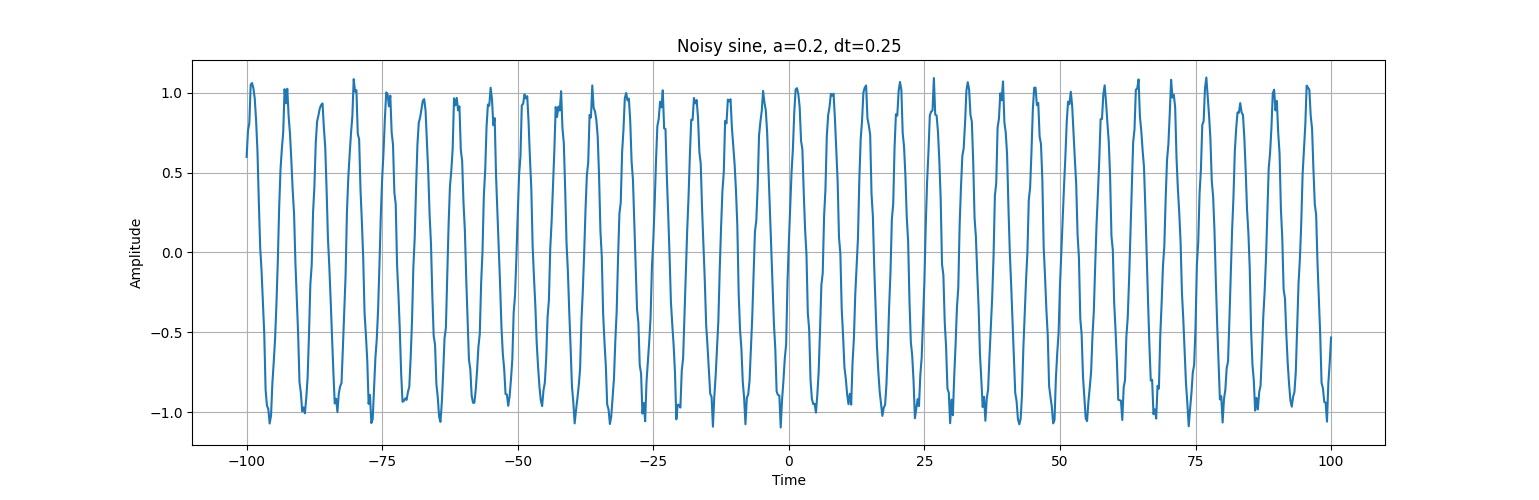
\includegraphics[scale=0.4]{1_noisy_sine.png}
        \captionsetup{skip=0pt}
        \caption{График зашумленного сигнала.}
        \label{fig:1ns}
    \end{figure}
    Найдем численную производную от данного сигнала, используя формулу поэлементного дифференцирования $$\dfrac{y(k+1)-y(k)}{dt},$$ после чего построим график.
    \begin{figure}[H]
        \centering
        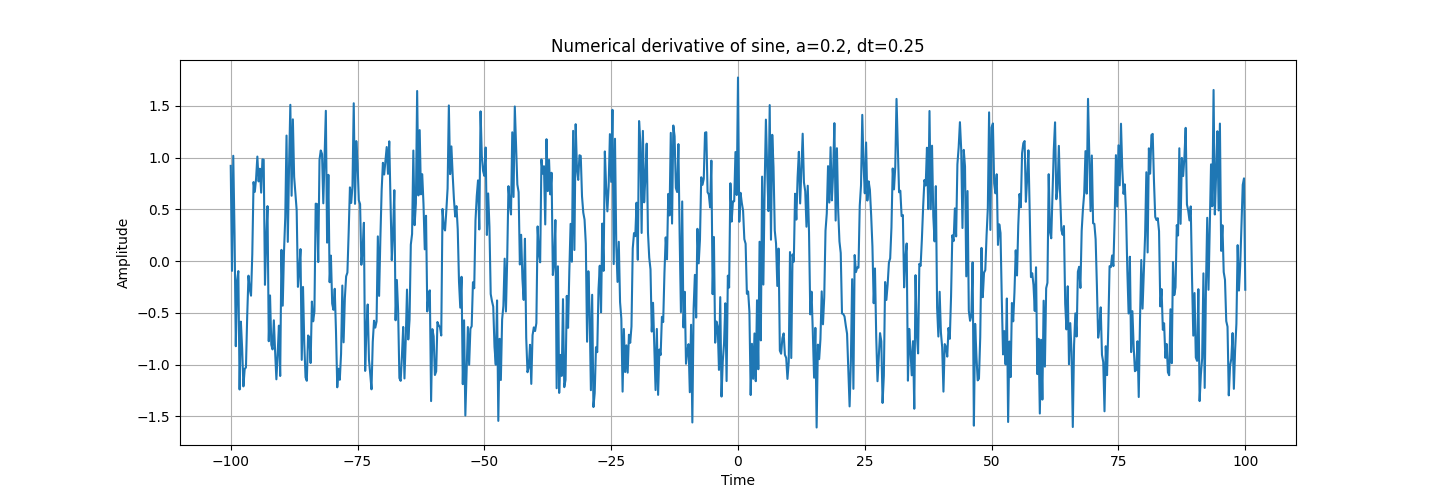
\includegraphics[scale=0.4]{1_numdiff_sine.png}
        \captionsetup{skip=0pt}
        \caption{Численная производная зашумленного сигнала.}
        \label{fig:1nds}
    \end{figure}
    Найдем спектральную производную от зашумленного сигнала. Для прямого и обратного преобразования Фурье будем использовать численное интегрирование (trapz). Чтобы
    превратить Фурье-образ сигнала в Фурье-образ производной, необходимо домножить результат преобразования Фурье на $2\pi i \nu$, где $\nu$ -- частота (Гц),
    таким образом получим формулу $$\mathcal{F}\left\{\frac{d}{dt}f\right\}=2\pi i \nu \mathcal{F}\left\{f\right\}.$$ Теперь остается только выполнить обратное преобразование Фурье, чтобы получить
    спектральную производную сигнала. Далее приведены графики вещественной и мнимой компонент Фурье-образа сигнала и его спектральной производной.
    \begin{figure}[H]
        \centering
        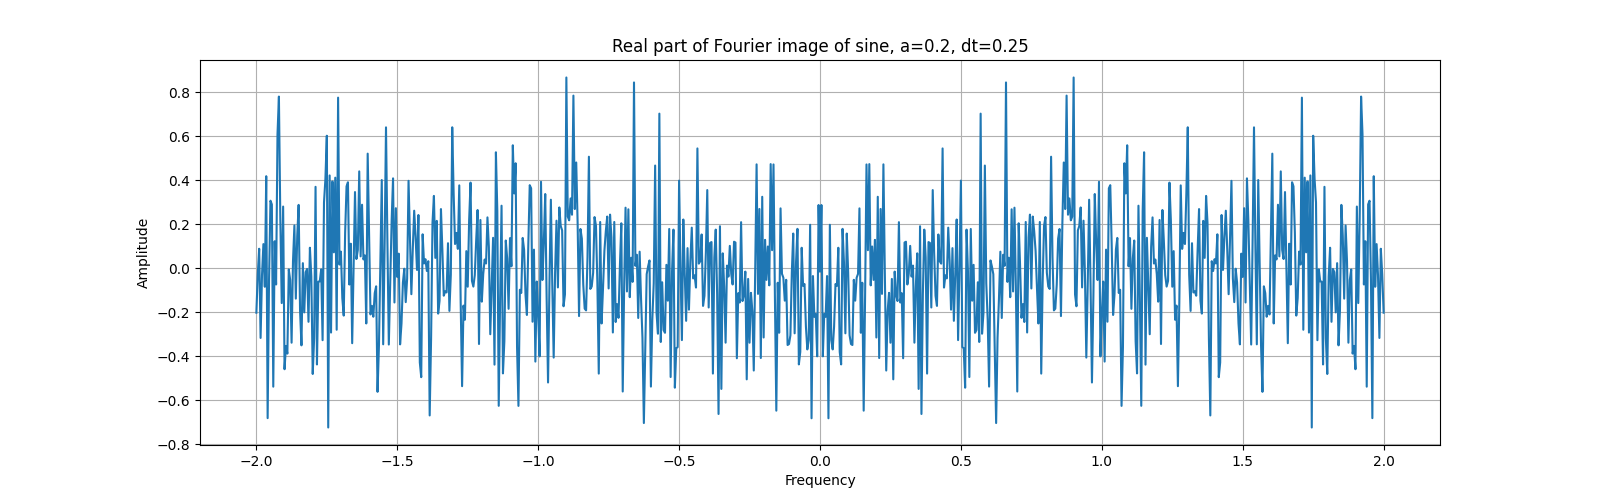
\includegraphics[scale=0.4]{1_re_fimg_sine.png}
        \captionsetup{skip=0pt}
        \caption{Вещественная компонента Фурье-образа зашумленного сигнала.}
        \label{fig:1refis}
    \end{figure}
    \begin{figure}[H]
        \centering
        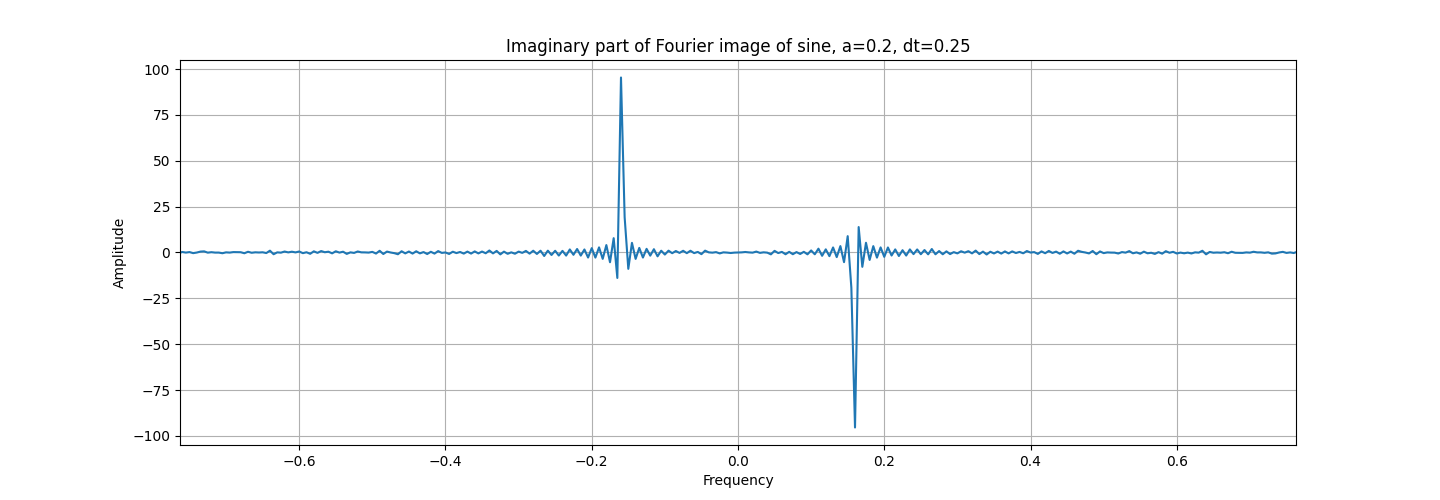
\includegraphics[scale=0.4]{1_im_fimg_sine.png}
        \captionsetup{skip=0pt}
        \caption{Мнимая компонента Фурье-образа зашумленного сигнала.}
        \label{fig:1imfis}
    \end{figure}
    \begin{figure}[H]
        \centering
        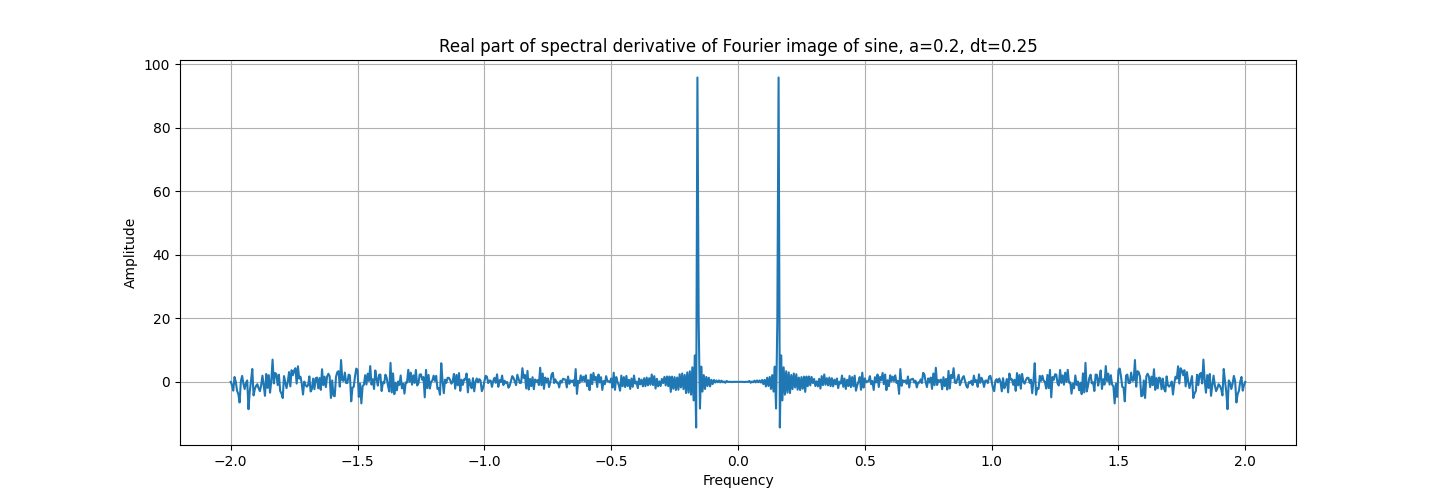
\includegraphics[scale=0.4]{1_re_spd_fimg_sine.png}
        \captionsetup{skip=0pt}
        \caption{Вещественная компонента спектральной производной Фурье-образа зашумленного сигнала.}
        \label{fig:1respdf}
    \end{figure}
    \begin{figure}[H]
        \centering
        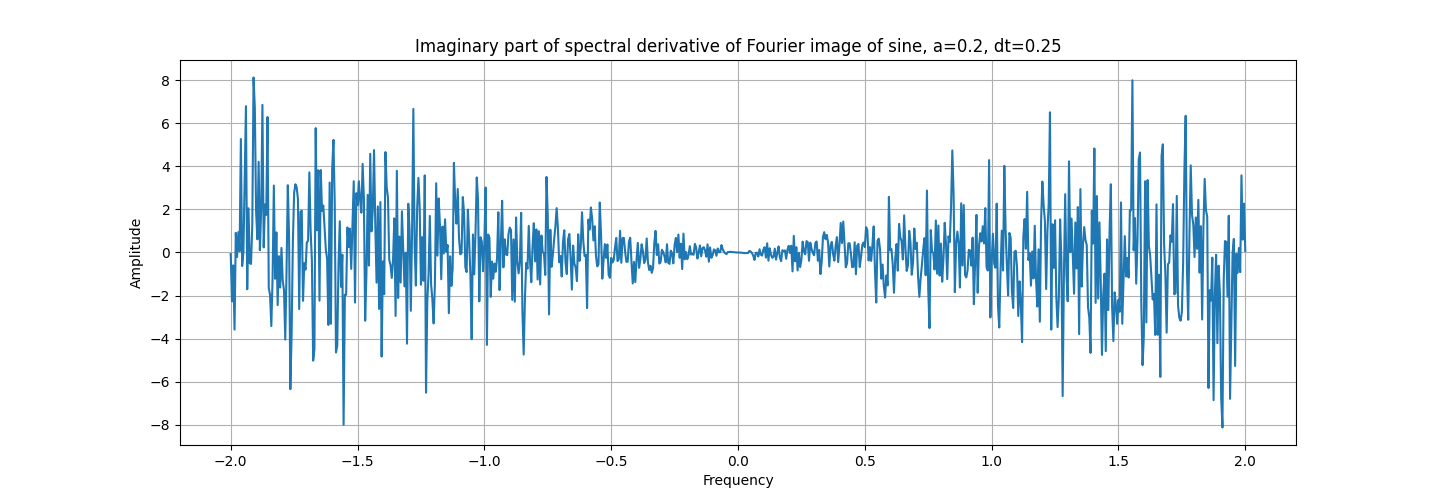
\includegraphics[scale=0.4]{1_im_spd_fimg_sine.png}
        \captionsetup{skip=0pt}
        \caption{Мнимая компонента спектральной производной Фурье-образа зашумленного сигнала.}
        \label{fig:1imspdf}
    \end{figure}


    Видим, что вещественная компонента Фурье-образа зашумленного сигнала и его спектральной производной симметричны относительно оси
    $OY$, а их мнимые компоненты относительно $OX$. Подобная симметричность сохраняется в не зависимости от четности исходной функции.


    На следующем рисунке приведен график вещественной части спектральной производной зашумленного сигнала, найденной с помощью численного интегрирования.
    Результат похож на численную производную, но с резкими возрастаниями амплитуд по краям. Данное поведение не зависит от наличия шума в сигнале или
    выбора шага дискретизации $dt$.
    \begin{figure}[H]
        \centering
        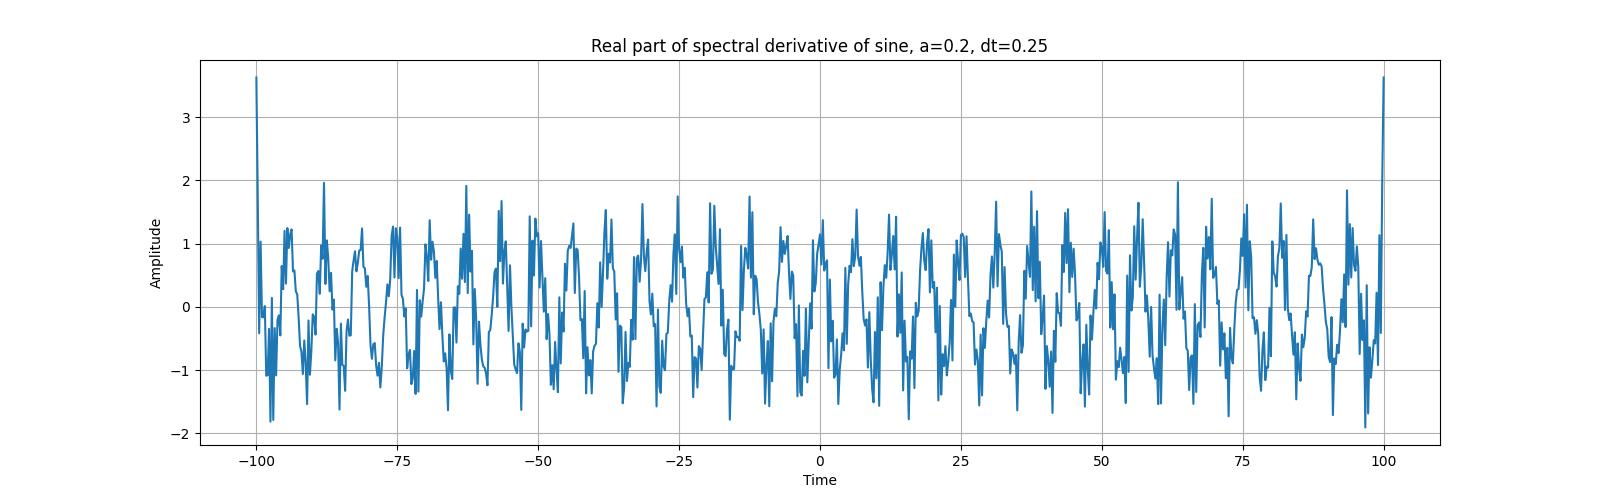
\includegraphics[scale=0.4]{1_re_specdiff_sine.png}
        \captionsetup{skip=0pt}
        \caption{Вещественная компонента спектральной производной зашумленного сигнала.}
        \label{fig:1respds}
    \end{figure}

    
    Теперь сравним график истинной производной $\cos{(t)}$ с графиками численной и спектральной производных зашумленного синуса.
    Оранжевым цветом обозначена спектральная производная, синим численная. Красным цветом выделена производная косинуса.
    \begin{figure}[H]
        \centering
        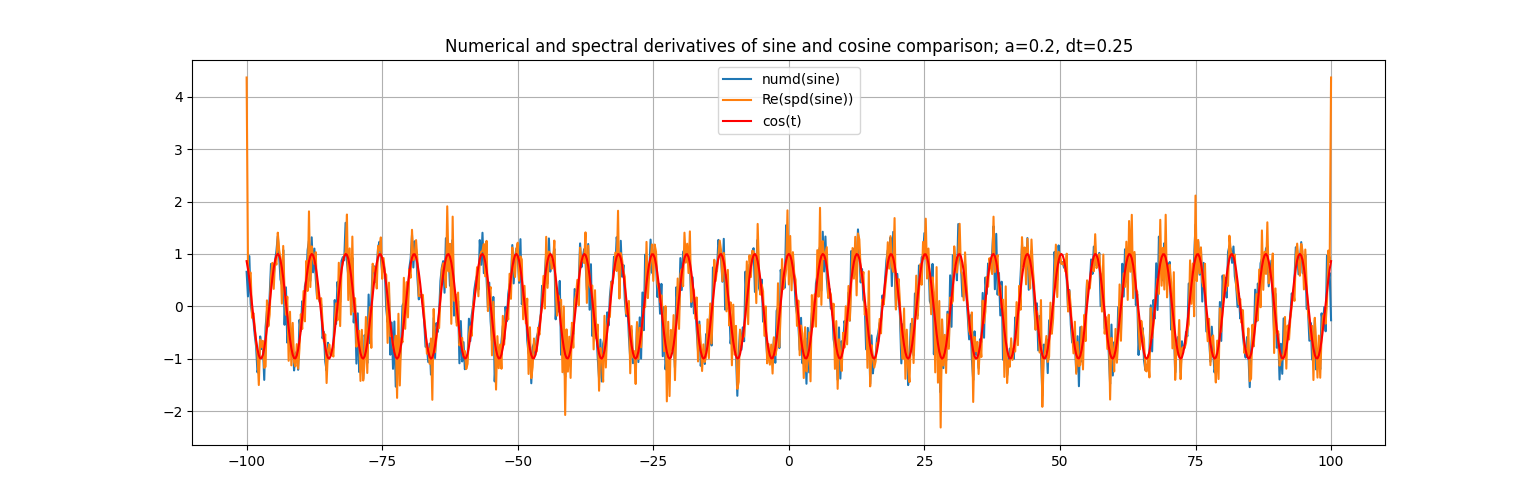
\includegraphics[scale=0.4]{1_css_comp.png}
        \captionsetup{skip=0pt}
        \caption{Сравнительный график производной $\cos{(t)}$ с численной и спектральной производными зашумленного $\sin{(t)}$.}
        \label{fig:css_comp}
    \end{figure}


    Графики численной и спектральной производных похожи друг на друга и на истинную производную косинуса (с разницей в смещении
    по фазе на $-\pi\div 2$). Спектральная производная имеет немного больше выбросов по сравнению с численной. Достаточно посмотреть
    на края графика спектральной производной и на ее амплитуды в точках максимума и минимума каждой волны.


    В ходе работы было выяснено, что при маленьком шаге $dt$ или при большом значении $a$ спектральная и численная производные
    становятся не похожи на истинную производную косинуса. По большей части на графиках видно белый шум. Если исходный сигнал
    имеет шумы, то его производная будет зашумлена сильнее. Наличие мнимой части у Фурье-образа не зависит от четности исходной
    функции. Более того, вещественные компоненты после преобразования Фурье симметричны относительно оси ординат, а мнимые относительно
    оси абсцисс.


    \subsection{Используемые программы}
    Все графики перового задания строились с помощью языка программирования Python с подключенной библиотекой matplotlib. Далее
    по ходу работы графики будут строиться той же программой. 
    \begin{lstlisting}[label=task1, caption={Файл с программой для построения графиков.}]
    import matplotlib.pyplot as plt

    def build_f(x, y, fz1=16,
                fz2=5, clr=None, ttl=None,
                grid=True, legend=False, xlab=None,
                ylab=None, xl1=None, xl2=None,
                yl1=None, yl2=None, lbl=None,
                ls='-', ticks=None, rot=None):
        plt.plot(x, y, color=clr, label=lbl, linestyle=ls)
        plt.xlabel(xlab)
        plt.ylabel(ylab)
        plt.xlim(xl1, xl2)
        plt.ylim(yl1, yl2)
        plt.xticks(ticks, rotation=rot)
        plt.title(ttl)
        plt.gcf().set_size_inches(fz1, fz2)
        plt.grid(grid)
        if legend:
            plt.legend()
        plt.show()
                
    def build_fs(x, y: list, colors: list=None,
                 labels: list=None, fz1=16, fz2=5,
                 ttl=None, grid=True, legend=False, 
                 xlab=None, ylab=None, xl1=None,
                 xl2=None, yl1=None, yl2=None,
                 ls:list=None, ticks=None, rot=None):
        if (y is None or len(y) <= 0):
            print('y is None or its len <= 0')
            return
        if (colors is None): colors = [None] * len(y)
        if (labels is None): labels = [None] * len(y)
        if (ls is None): ls = ['-'] * len(y)
        
        for k in range(len(y)):
            plt.plot(x, y[k], color=colors[k],
                     label=labels[k], linestyle=ls[k])
        plt.xlabel(xlab)
        plt.ylabel(ylab)
        plt.xlim(xl1, xl2)
        plt.ylim(yl1, yl2)
        plt.xticks(ticks, rotation=rot)
        plt.title(ttl)
        plt.gcf().set_size_inches(fz1, fz2)
        plt.grid(grid)
        if legend: plt.legend()
        plt.show()
    \end{lstlisting}


    \newpage
    Для нахождения Фурье-образа и производных использовалась библиотека numpy.
    \begin{lstlisting}[label=task1_2, caption={Программа для вычисления Фурье-образа численным интегрированием и производных.}]
    import numpy as np

    def trapz(y, t, v):
        Y = []
        for k in v:
            Y_k = np.trapz(y * np.exp(-1j * 2 * np.pi * k * t), t)
            Y.append(Y_k)
        return Y

    def undo_trapz(Y, t, v):
        y = []
        for k in t:
            y_k = np.trapz(Y * np.exp(1j * 2 * np.pi * k * v), v)
            y.append(y_k)
        return y

    def numerical_diff(y, dt):
        ndiff = []
        for k in range(len(y) - 1):
            ndiff_k = (y[k + 1] - y[k]) / dt
            ndiff.append(ndiff_k)
        return ndiff

    def spectral_diff(y, t, v):
        Y = trapz(y, t, v)
        dY = 2 * np.pi * 1j * v * Y
        spdiff = undo_trapz(dY, t, v)
        return spdiff, Y, dY
    \end{lstlisting}


    Программа, где используются написанные функции и задаются необходимые параметры, расположена ниже.
    \begin{lstlisting}
    import numpy as np

    import build_func as bf
    import fourier_math as fm

    T = 200
    dt = 0.25
    t = np.arange(-T / 2, T / 2 + dt, dt)
    y = np.sin(t)

    a = 0.2
    y += a * (np.random.rand(len(t)) - 0.5)

    ndsin = fm.numerical_diff(y, dt)
    ndsin.append(y[-1] / 2)

    V = 1 / dt
    dv = 1 / T
    v = np.arange(-V / 2, V / 2 + dv, dv)
    spdsin, Y, dY = fm.spectral_diff(y, t, v)
    tdcos = -np.sin(t)

    bf.build_f(t, y, ttl=f'Noisy sine, a={a}, dt={dt}',
               xlab='Time', ylab='Amplitude')
    bf.build_f(v, np.array(Y).real,
               ttl=f'Real part of Fourier image of sine, a={a}, dt={dt}',
               xlab='Frequency', ylab='Amplitude')
    bf.build_f(v, np.array(Y).imag,
             ttl=f'Imaginary part of Fourier image of sine, a={a}, dt={dt}',
             xlab='Frequency', ylab='Amplitude', xl1=-0.763, xl2=0.763)
    bf.build_f(v, dY.real,
               ttl=f'Real part of spectral derivative of Fourier image of sine, a={a}, dt={dt}',
               xlab='Frequency', ylab='Amplitude')
    bf.build_f(v, dY.imag,
               ttl=f'Imaginary part of spectral derivative of Fourier image of sine, a={a}, dt={dt}',
               xlab='Frequency', ylab='Amplitude')

    bf.build_f(t, ndsin,
               ttl=f'Numerical derivative of sine, a={a}, dt={dt}',
               xlab='Time', ylab='Amplitude')
    bf.build_f(t, np.array(spdsin).real,
            ttl=f'Real part of spectral derivative of sine, a={a}, dt={dt}',
            xlab='Time', ylab='Amplitude')
    bf.build_fs(t, y=[ndsin, np.array(spdsin).real, tdcos],
                colors=[None, None, 'r'], legend=True, 
                labels=['Num. der. of sine', 'Re. spec. der. of sine', 'True der. of cosine'],
                ttl=f'True der. of cosine, num. der. of sine and spec. der. of sine comparison; a={a}, dt={dt}')
    \end{lstlisting}
\end{document}